\chapter{反函数和反三角函数}
1.导数与反函数\\
如果$f$在其定义域$(a,b)$上可导且满足以下条件中的任意一条:\\
(1)对于所有的在$(a,b)$中的$x$, $f'(x)>0$;\\
(2)对于所有的在$(a,b)$中的$x$, $f'(x)<0$;\\
(3)对于所有的在$(a,b)$中的$x$, $f'(x)\geqslant 0$且对于有限个数的$x$, $f'(x)=0$;\\
(4)对于所有的在$(a,b)$中的$x$, $f'(x)\leqslant 0$且对于有限个数的$x$, $f'(x)=0$.\\
则$f$有反函数.\\[2ex]

反函数的导数:
\begin{center}
\framebox{如果$\displaystyle y=f^{-1}(x)$, 则$\displaystyle\frac{\dif y}{\dif x}=\frac{1}{f'(y)}=\frac{1}{f'(f^{-1}(x))}$}\\[1ex]
\end{center}
例.\\
\phantom{例}$h(x)=x^3$, 如果$y=h^{-1}(x)$, 求$\displaystyle\frac{\dif y}{\dif x}$\\
推导过程:\\
$\displaystyle\frac{\dif y}{\dif x}=\frac{1}{f'(y)}=\frac{1}{(y^3)'}=\frac{1}{3y^2}$\\
$\displaystyle y=h^{-1}(x)=x^{\frac{1}{3}}$\\
$\displaystyle\therefore\frac{\dif y}{\dif x}=\frac{1}{3y^2}=\frac{1}{3x^{\frac{2}{3}}}$\\[2ex]

2.反三角函数\\
(1)$\sin^{-1}$是奇函数; 其定义域为$[-1,1]$, 值域为$\displaystyle[-\frac{\pi}{2},\frac{\pi}{2}]$\\[1ex]
(2)$\displaystyle\frac{\dif }{\dif x}\sin^{-1}(x)=\frac{1}{\sqrt{1-x^2}}$, 其中$-1<x<1$.\\[1ex]
如图:
\begin{figure}[H]
\centering
	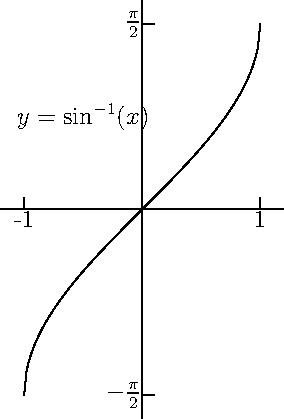
\includegraphics{asin.pdf}
\end{figure}
例.\\
\phantom{例}$\displaystyle\frac{\dif}{\dif x}\sin^{-1}(x)$\\
推导过程:\\

(3)$\cos^{-1}$既不是偶函数也不是奇函数; 其定义域为$[-1,1]$, 值域为$[0,\pi]$.\\[1ex]
(4)$\displaystyle\frac{\dif }{\dif x}\cos^{-1}(x)=-\frac{1}{\sqrt{1-x^2}}$, 其中$-1<x<1$.\\[1ex]
如图:
\begin{figure}[H]
\centering
	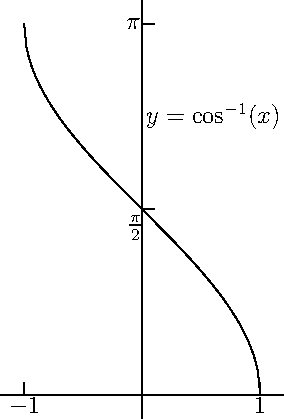
\includegraphics{acos.pdf}
\end{figure}
(5)$\tan^{-1}$是奇函数; 其定义域是$\mathbb{R}$且值域是$\displaystyle(-\frac{\pi}{2},\frac{\pi}{2})$.\\[1ex]
(6)对于所有的实数$x$, $\displaystyle\frac{\dif }{\dif x}\tan^{-1}(x)=\frac{1}{1+x^2}$.\\[1ex]
如图:
\begin{figure}[H]
\centering
	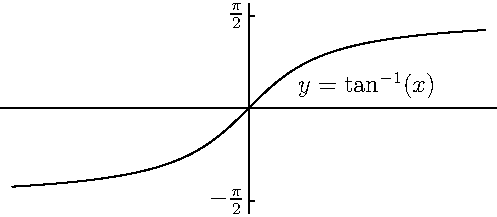
\includegraphics{atan.pdf}
\end{figure}
(7)$\cot^{-1}$既不是奇函数也不是偶函数; 其定义域为$\mathbb{R}$且值域是$(0,\pi)$\\[1ex]
(8)对于所有的实数$x$, $\displaystyle\frac{\dif }{\dif x}\cot^{-1}(x)=-\frac{1}{1+x^2}$.\\[1ex]
\begin{figure}[H]
\centering
	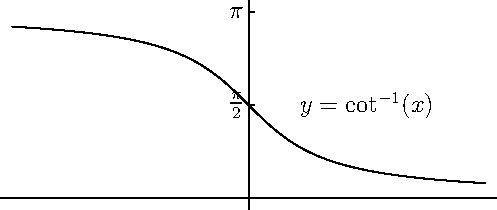
\includegraphics{acot.pdf}
\end{figure}
(9)$\sec^{-1}$既不是奇函数也不是偶函数; 其定义域是$(-\infty,-1]\cup[1,\infty)$且值域是$\displaystyle[0,\frac{\pi}{2})\cup(\frac{\pi}{2},\pi]$.\\[1ex]
(10)对于$x>1$或$x<-1$, $\displaystyle\frac{\dif }{\dif x}\sec^{-1}(x)=\frac{1}{|x|\sqrt{x^2-1}}$.\\[1ex]
\begin{figure}[H]
\centering
	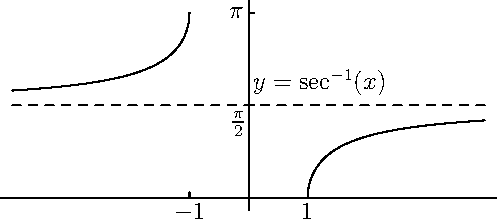
\includegraphics{asec.pdf}
\end{figure}

(11)$\csc^{-1}$是奇函数; 其定义域为$(-\infty,-1]\cup[1,\infty)$且值域是$\displaystyle[-\frac{\pi}{2},0)\cup(0,\frac{\pi}{2}]$.\\[1ex]
(12)对于$x>1$或$x<-1$, $\displaystyle\frac{\dif }{\dif x}\csc^{-1}(x)=-\frac{1}{|x|\sqrt{x^2-1}}$.\\[2ex]
\begin{figure}[H]
\centering
	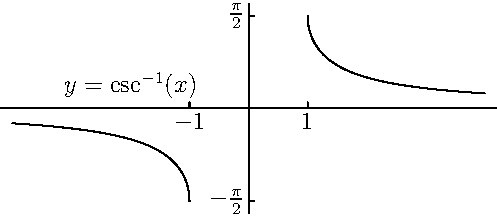
\includegraphics{acsc.pdf}
\end{figure}\vspace{2ex}

4.计算反三角函数\\
化简形如$\sin^{-1}(\sin(\alpha))$的三角函数:\\
\phantom{(1)}获取指定角$\alpha$的参照角\\
\phantom{(1)}找到反三角函数定义域中拥有该参照角的角\\
\phantom{(1)}确定该角的正弦值与$\alpha$参照角的正弦值符号一致\\[2ex]

5.反双曲函数\\
(1)$\sinh^{-1}$是奇函数; 其定义域和值域都是$\mathbb{R}$.\\[1ex]
(2)对于所有的实数$x$, $\displaystyle\frac{\dif }{\dif x}\sinh^{-1}(x)=\frac{1}{\sqrt{x^2+1}}$.\\[1ex]
(3)$\cosh^{-1}$既不是奇函数也不是偶函数; 其定义域是$[1,\infty)$且值域是$[0,\infty)$.\\[1ex]
(4)对于$x>1$, $\displaystyle\frac{\dif }{\dif x}\cosh^{-1}(x)=\frac{1}{\sqrt{x^2-1}}$.\\[1ex]
